\section{MapReduce Service}\label{mapreduce_service}
This section will explore the \textbf{logical design of the MapReduce operation performed as a Grid Service}. The process is modeled using three \textbf{Petri Nets}, each one \textbf{providing the point of view of one among the possible entities types involved}: Map Worker, Reduce Worker and MapReduce Master.

Every Petri Net that will be presented \textbf{assumes that the Resources' retrieval process} (viewed in \textit{figure \ref{fig:use_cases_satisfaction_node_contribution}}) \textbf{has already been performed, allowing to focus on the actual MapReduce process itself}.
Furthermore, in every Petri Net snapshot provided, transitions that can be transitioned (in that particular configuration of the places) are highlighted in red to facilitate its understanding.
  
\subsection{Map Worker}
The process starts with the Map Worker \textbf{establishing a connection with the MapReduce Master} (\textit{figure \ref{fig:map_worker_petri_net_1}}).

\vspace{5mm}

\begin{figure}[!ht]
    \centering
    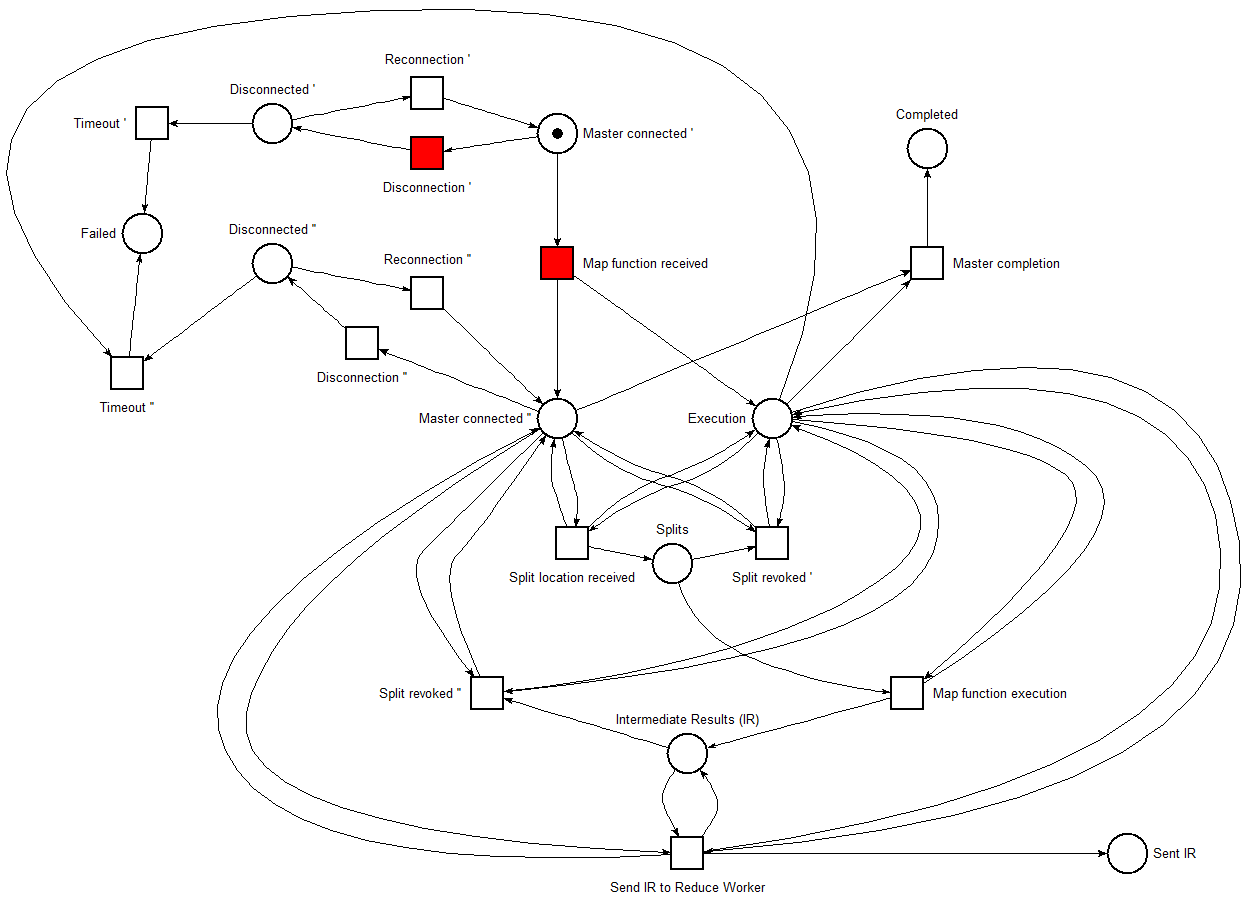
\includegraphics[width=\linewidth]{document/chapters/chapter_5/images/map_worker_petri_net_1.png}
    \caption{Map Worker - Start}
    \label{fig:map_worker_petri_net_1}
\end{figure}

Ignoring, for the moment, the \textit{Disconnection'} transition, \textbf{the Map Worker receives the Map function from the MapReduce Master}, obtaining a token for the \textit{Execution} place and one for the \textit{Master Connected''} place. The \textbf{distinction between the concepts of connection and execution} is useful here since \textbf{it is not necessary to be connected to the Grid Master in order to execute the map function}; through this distinction, Resources can be used efficiently even if a temporary disconnection occurs.

\textit{Figure \ref{fig:map_worker_petri_net_2}} shows how, \textbf{once the map function is received, the MapReduce Master starts to send the location where the data splits can be retrieved}; the Map Worker retrieves the specified data and \textbf{applies the map function to it producing the intermediate results (IR) as output}.

\vspace{5mm}

\begin{figure}[!ht]
    \centering
    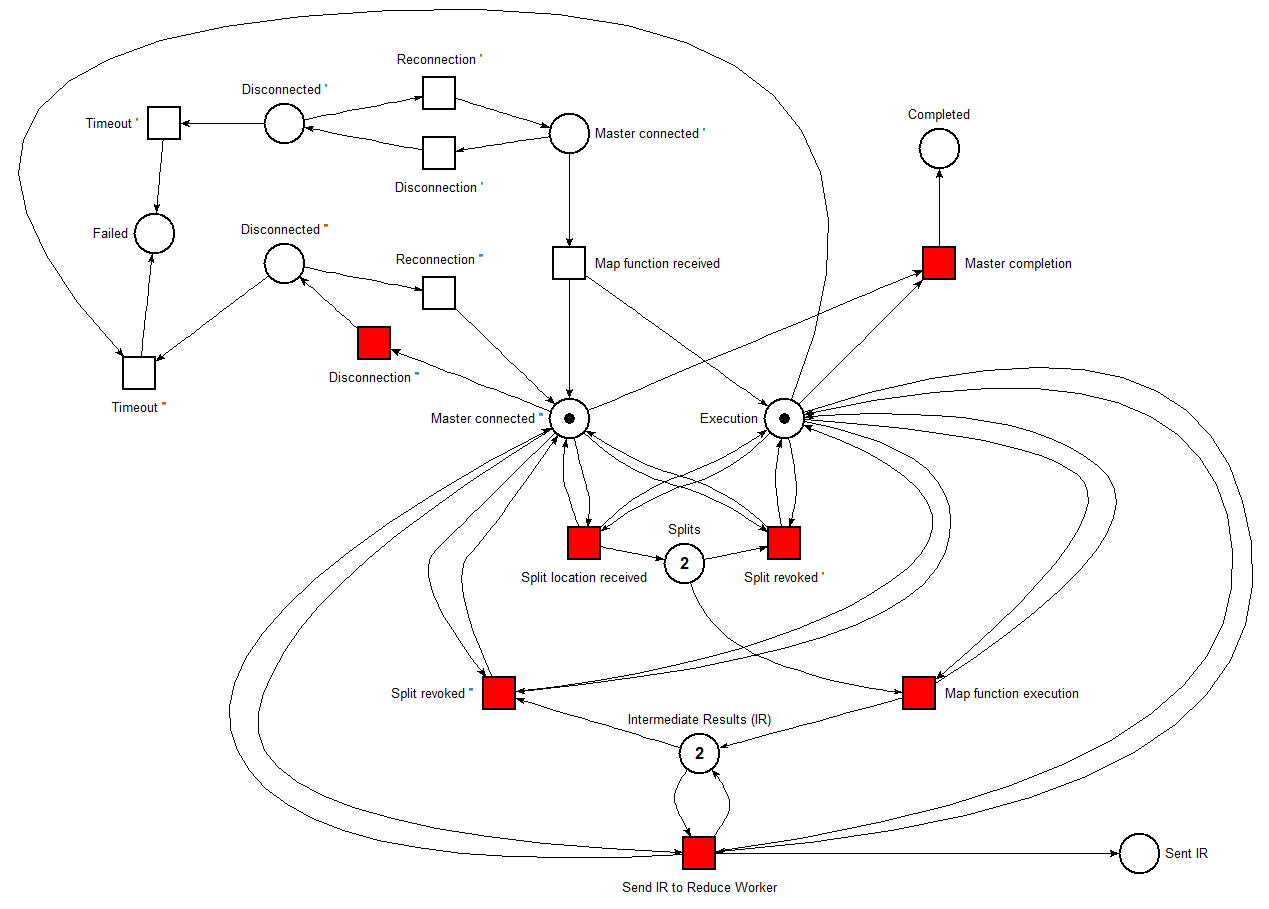
\includegraphics[width=\linewidth]{document/chapters/chapter_5/images/map_worker_petri_net_2.png}
    \caption{Map Worker - Mapping}
    \label{fig:map_worker_petri_net_2}
\end{figure}

As can be seen from the operations executed, \textbf{the Map Worker follows the instructions received by the MapReduce Master}. While mapping, \textbf{a data split can be assigned to multiple Map Workers}, in order to increase fault tolerance; as a direct consequence, \textbf{it is possible that a received split location is mapped by another Map Worker}. \textbf{Once the IR is already obtained on a particular split, the Map Worker sends a split revoked' instruction to every Map Worker assigned to that split}. The two different split revoked transitions possess a conceptual difference:
\begin{itemize}
    \item \textit{\textbf{Split revoked'}}\\
    Here, \textbf{the Map Worker that receives this instruction cannot possibly have applied the map function to the split}, since the split revoked instruction is received only after the IR (produced by the mapping of that particular split) is reduced by a Reduce Worker. \textbf{Practically speaking, the Map Worker drops the split, removing it from memory or avoiding downloading it entirely}.
    \item \textit{\textbf{Split revoked''}}\\
    In this situation, \textbf{the Map Worker already performed the map operation on the considered split}. Whether the IR that will be used for the reduce operation is actually the one locally produced or not is irrelevant; the direct consequence of receiving a split revoked instruction here is to \textbf{remove from memory the IR}. This is because \textbf{the MapReduce Master can ask multiple times to the Map Worker to send the IR to a Reduce Worke}r (\textit{figure \ref{fig:map_worker_petri_net_3}}), \textbf{requiring to maintain in memory} (or on disk) \textbf{the IR until the split revoked instruction is received}.
\end{itemize}

\vspace{2mm}

\begin{figure}[!ht]
    \centering
    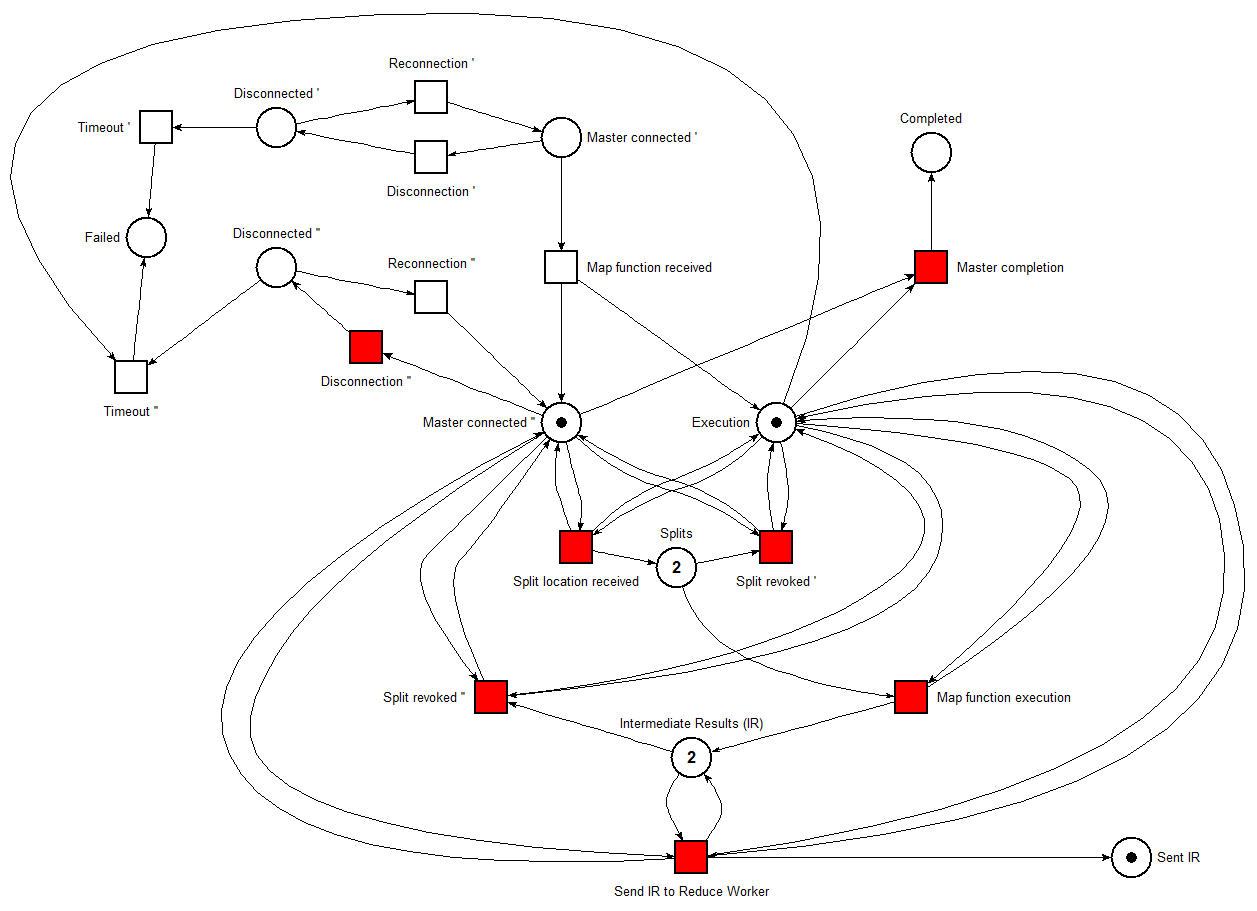
\includegraphics[width=\linewidth]{document/chapters/chapter_5/images/map_worker_petri_net_3.png}
    \caption{Map Worker - Intermediate Result sent}
    \label{fig:map_worker_petri_net_3}
\end{figure}

\vspace{2mm}

At any given time, \textbf{the Map Worker can lose the connection with the MapReduce Master} (\textit{Disconnection'} and \textit{Disconnection''} transitions); \textbf{before receiving the Map function, the process is necessarily locked until the connection is established once again or a timeout is reached}, leading to a local \textbf{failure}. On the contrary, \textbf{if the token on the execution place is present, the Map Worker is still able to apply the map function on a split that is locally available even though it is in a disconnected state}; on the other hand, \textbf{a timeout leading to a failure would also remove the execution token}, effectively stopping the entire process.

When the MapReduce operation is completed, \textbf{the Master will send a completion instruction} that will result in the removal of the connection and execution tokens, \textbf{correctly concluding the execution} (\textit{figure \ref{fig:map_worker_petri_net_4}}).

\begin{figure}[!ht]
    \centering
    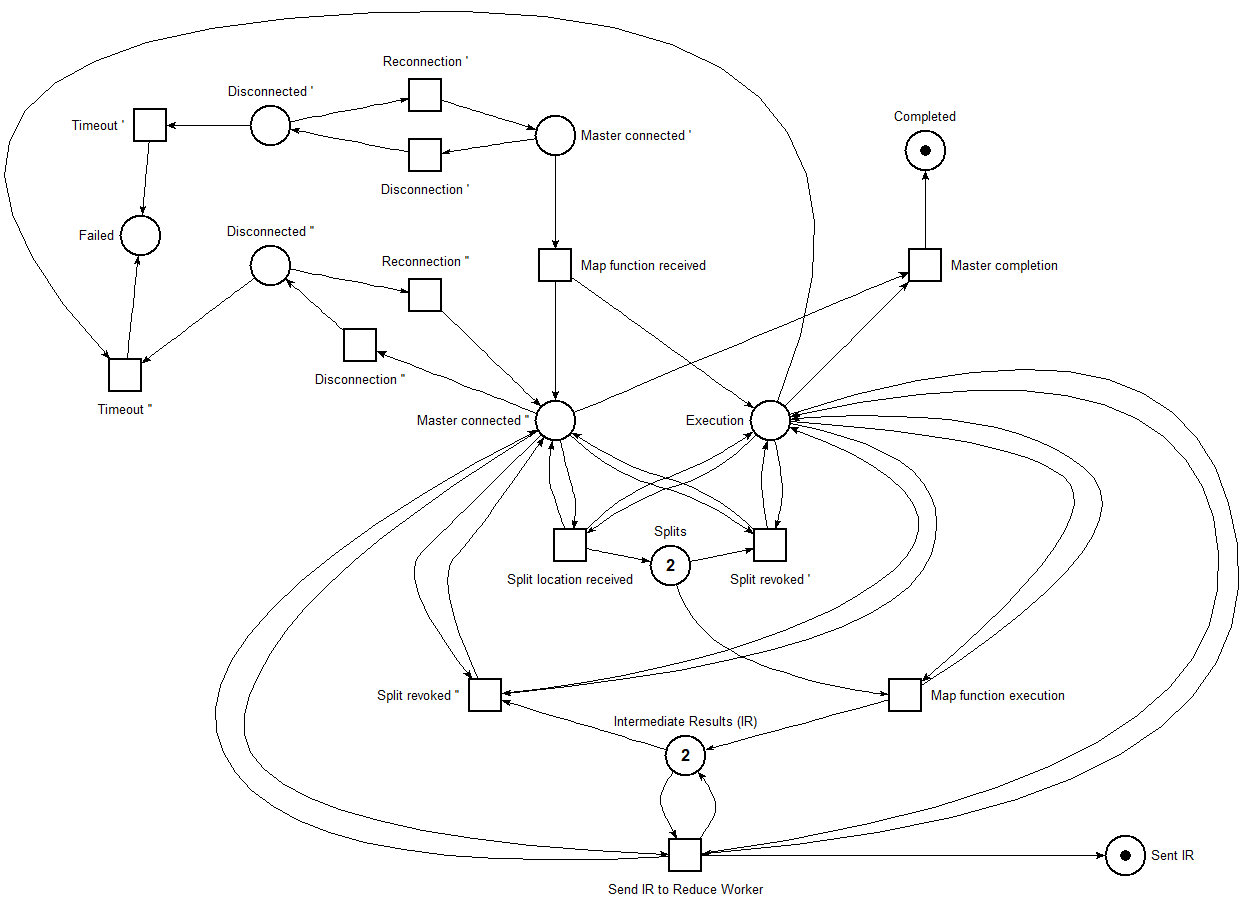
\includegraphics[scale=0.45]{document/chapters/chapter_5/images/map_worker_petri_net_4.png}
    \caption{Map Worker - Completion}
    \label{fig:map_worker_petri_net_4}
\end{figure}

\subsection{Reduce Worker}
As the Map Worker's process, \textbf{a connection to the MapReduce Master is established and a reduce function is received, gaining a connection token and an execution token} (used for the same Resources' utilization optimization principle); \textbf{as before, a disconnection can occur and, if a timeout is reached, the process ends with a failure}.

\textbf{The MapReduce Master sends the data about which IRs constitute a region} (\textit{figure \ref{fig:reduce_worker_petri_net_1}} shows an example of a region composed by 10 IRs); \textbf{the Reduce Worker also receives}, progressively, \textbf{the IRs from the Map Workers that have completed the execution of a map function} and are instructed to send said data to that particular Reduce Worker. \textbf{Once all the IRs belonging to a region are received}, the Reduce Worker performs the \textbf{reduce function} on said data, producing a \textbf{result that is momentarily stored locally}.

\begin{figure}[!ht]
    \centering
    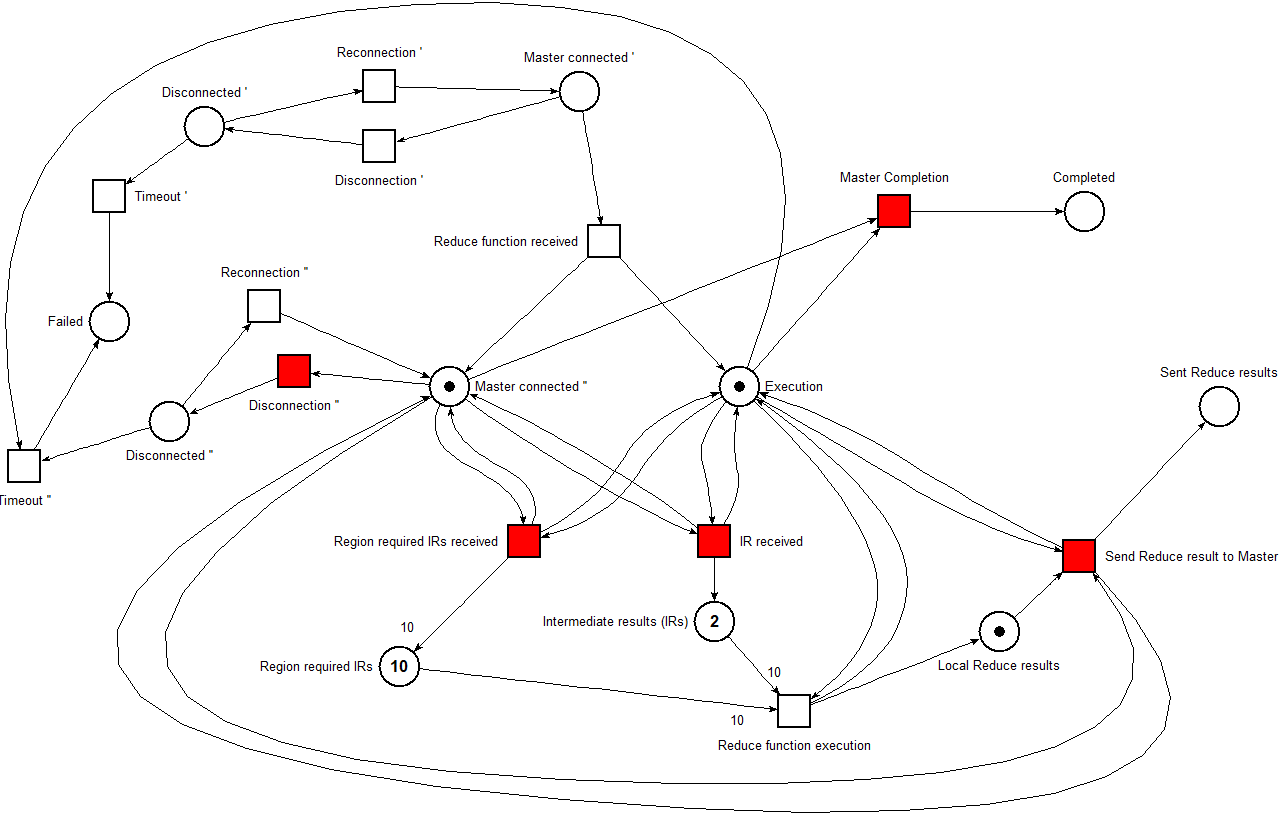
\includegraphics[scale=0.44]{document/chapters/chapter_5/images/reduce_worker_petri_net_1.png}
    \caption{Reduce Worker - Local result}
    \label{fig:reduce_worker_petri_net_1}
\end{figure}

\textbf{A result correctly sent to the Master is deleted locally}. \textbf{A Reduce Worker handles multiple regions until the MapReduce process is completed}; once the Master sends to the Worker a completion instruction the execution ends correctly (\textit{figure \ref{fig:reduce_worker_petri_net_2}}).

\begin{figure}[!ht]
    \centering
    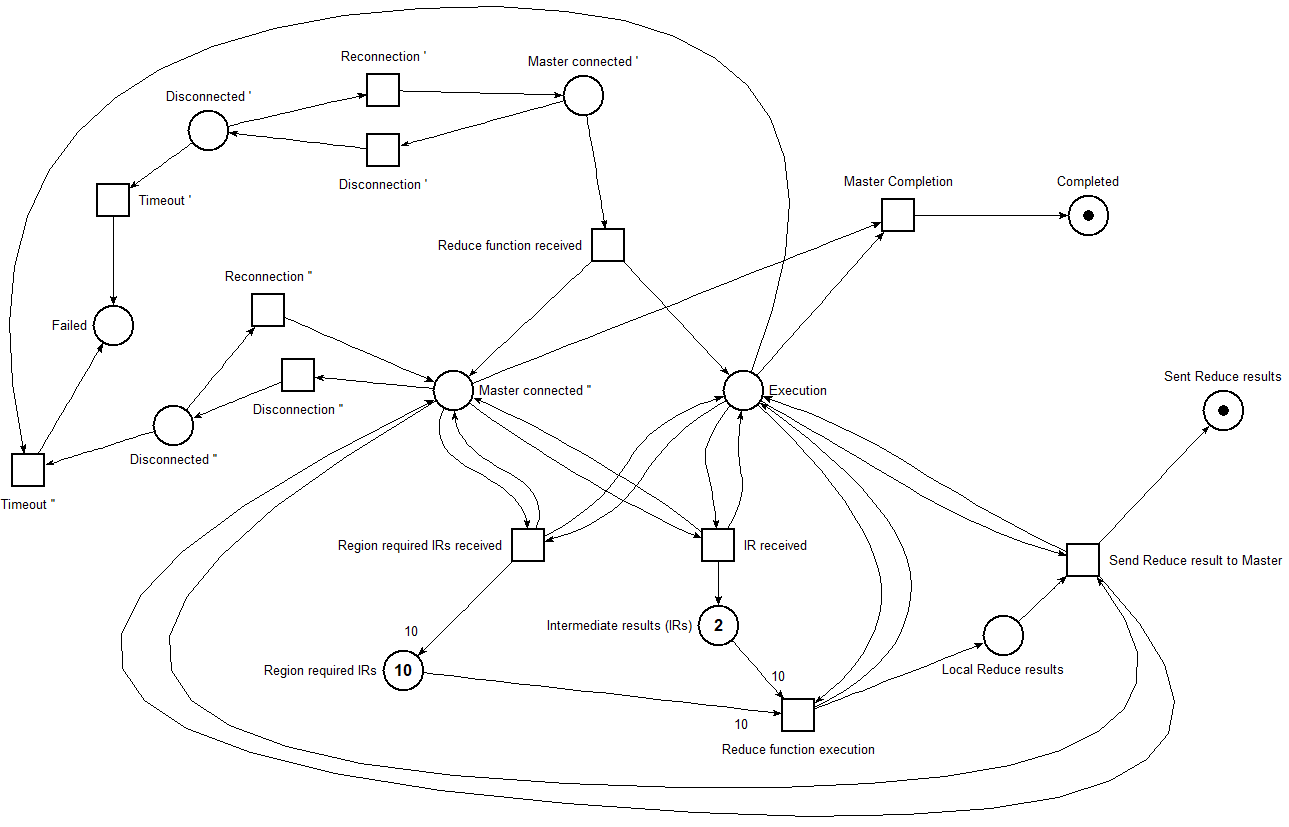
\includegraphics[scale=0.44]{document/chapters/chapter_5/images/reduce_worker_petri_net_2.png}
    \caption{Reduce Worker - Completion}
    \label{fig:reduce_worker_petri_net_2}
\end{figure}

\subsection{MapReduce Master}
\textbf{The Petri Net} describing the process performed by the MapReduce Master \textbf{focuses only on a single region}, meaning that \textbf{this operation needs to be performed (concurrently) for each data region}. 
\begin{figure}[!ht]
    \centering
    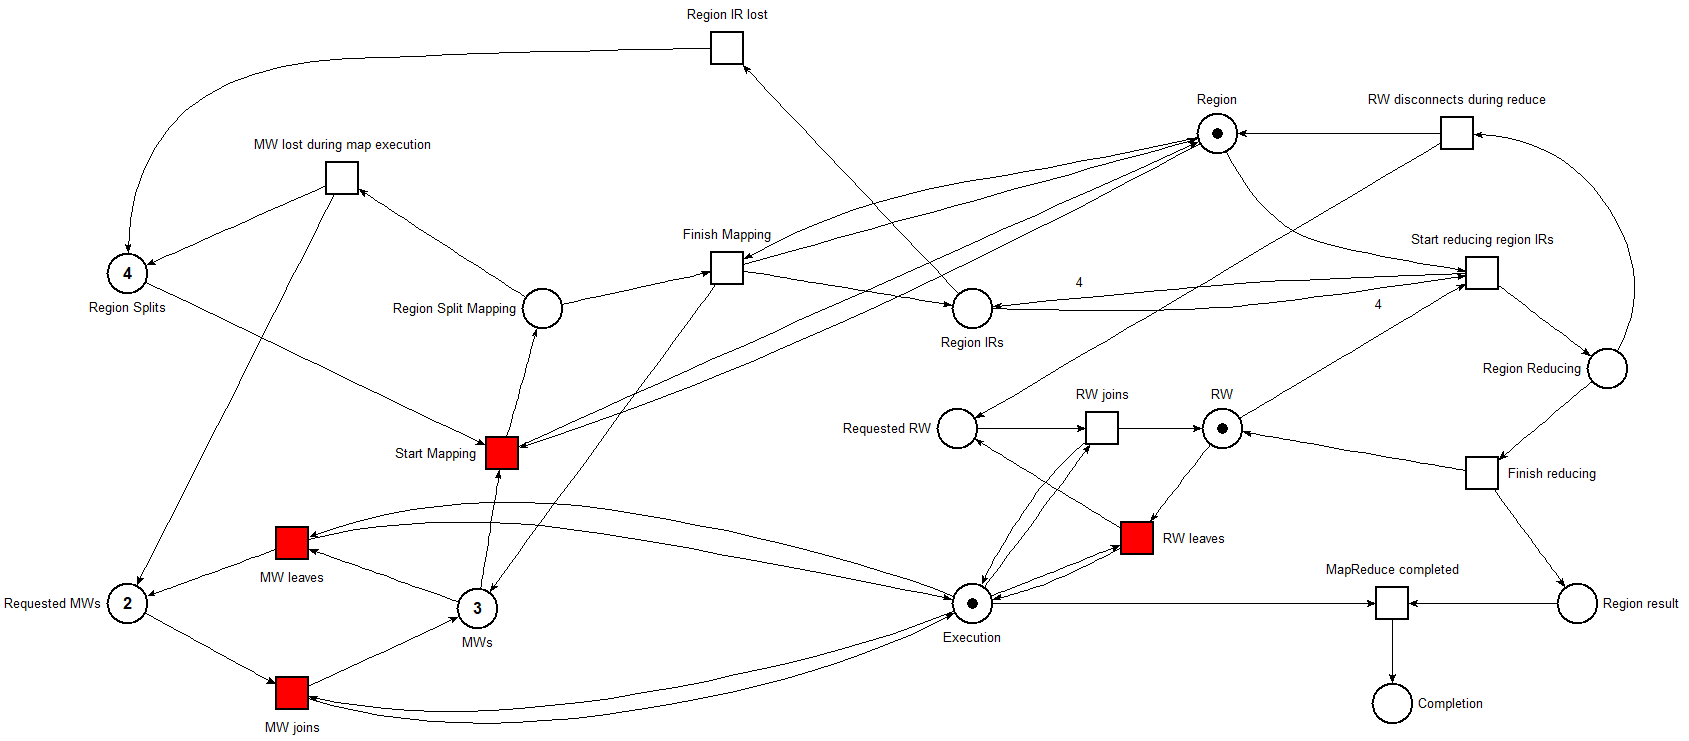
\includegraphics[width=\linewidth]{document/chapters/chapter_5/images/master_petri_net_1.png}
    \caption{MapReduce Master - Recruitment}
    \label{fig:master_petri_net_1}
\end{figure}

For this particular example, the region is constituted by 4 splits and the Customer required a quantity of Resources that resulted in the Contribution of 5 Map Workers; \textbf{a region is handled by a single Reduce Worker}, so there is only one token representing it.

Initially, \textbf{the Map and Reduce Workers are required but not connected} (\textit{Requested MWs} and \textit{Requested RW} places); they can \textbf{transition to a connected state} but, if something goes wrong, they \textbf{can also disconnect}. \textit{Figure \ref{fig:master_petri_net_1}} shows a situation where 3 Map Workers and the Reduce Worker have joined. \textbf{Workers can continue to join and leave until the MapReduce computation for the region is completed}, removing the execution token.

\textbf{Having at least one MW available, the mapping process can begin} (\textit{figure \ref{fig:master_petri_net_2}}). A \textbf{split} belonging to the region is \textbf{assigned to an available MW which will perform the Map operation on it} (it is assumed that the Worker possesses the map function, abstracted for simplicity). If the mapping happens successfully, \textbf{the region's IRs are accumulated}; \textbf{in case that a Map Worker is lost} during the map execution, \textbf{the split needs to be computed by another Worke}r and is \textbf{placed back in the \textit{Regions splits} place} (and the another token in the requested MWs is also placed).
It can also happen that \textbf{a region's IR is lost due to the disconnection of the Map Worker that is still keeping the result in memory}; this occurrence also \textbf{adds again said split in the \textit{Region splits}} that still needs to be mapped (since its IR is unreachable).

\begin{figure}[!ht]
    \centering
    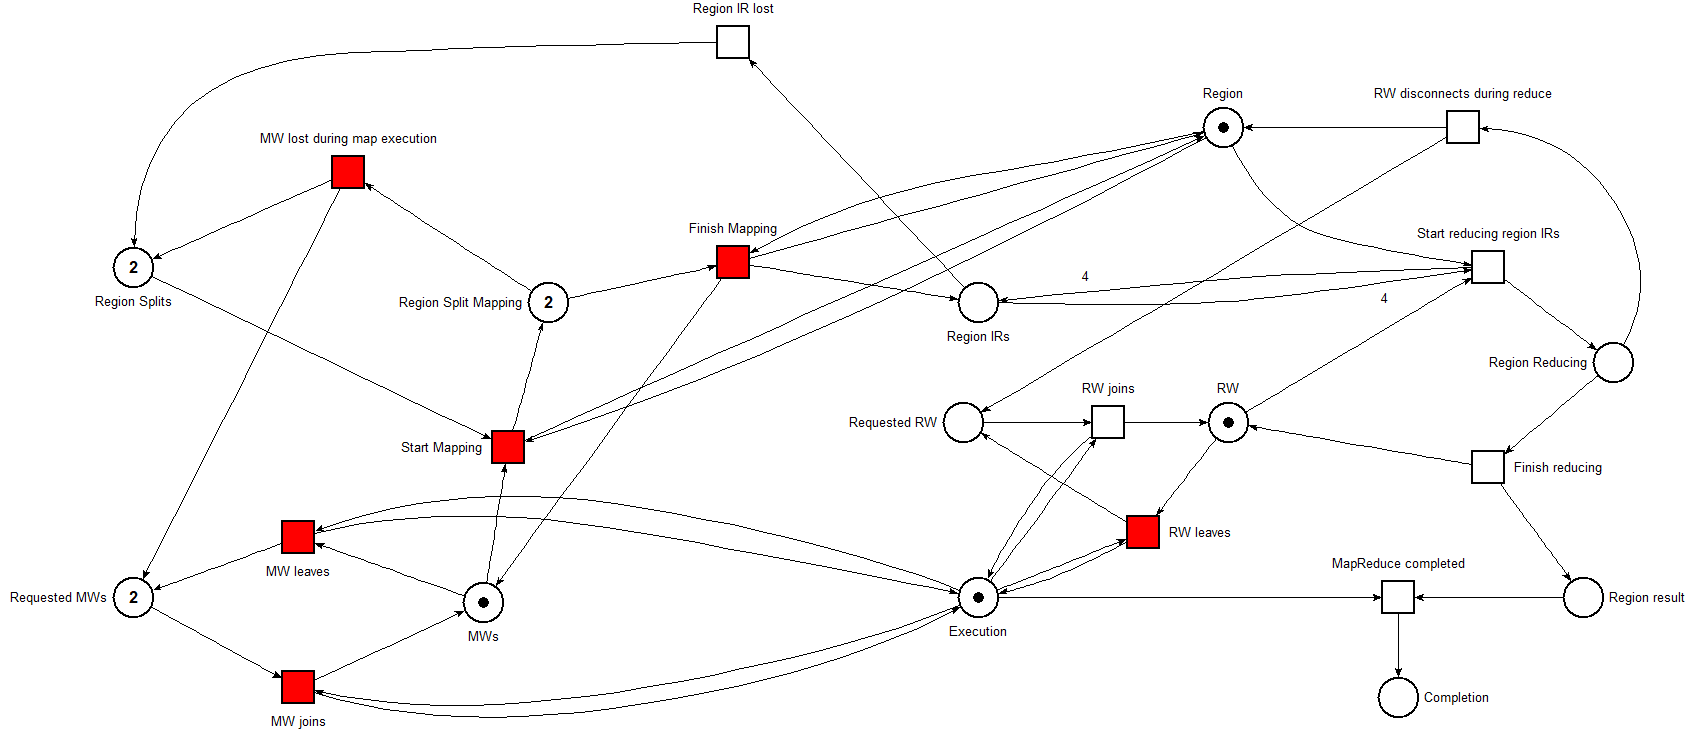
\includegraphics[width=\linewidth]{document/chapters/chapter_5/images/master_petri_net_2.png}
    \caption{MapReduce Master - Mapping process}
    \label{fig:master_petri_net_2}
\end{figure}

Once \textbf{all the region's split are mapped} to intermediate results (\textit{figure \ref{fig:master_petri_net_3}}), \textbf{the reduce process can start} (assuming that a RW is connected).

\begin{figure}[!ht]
    \centering
    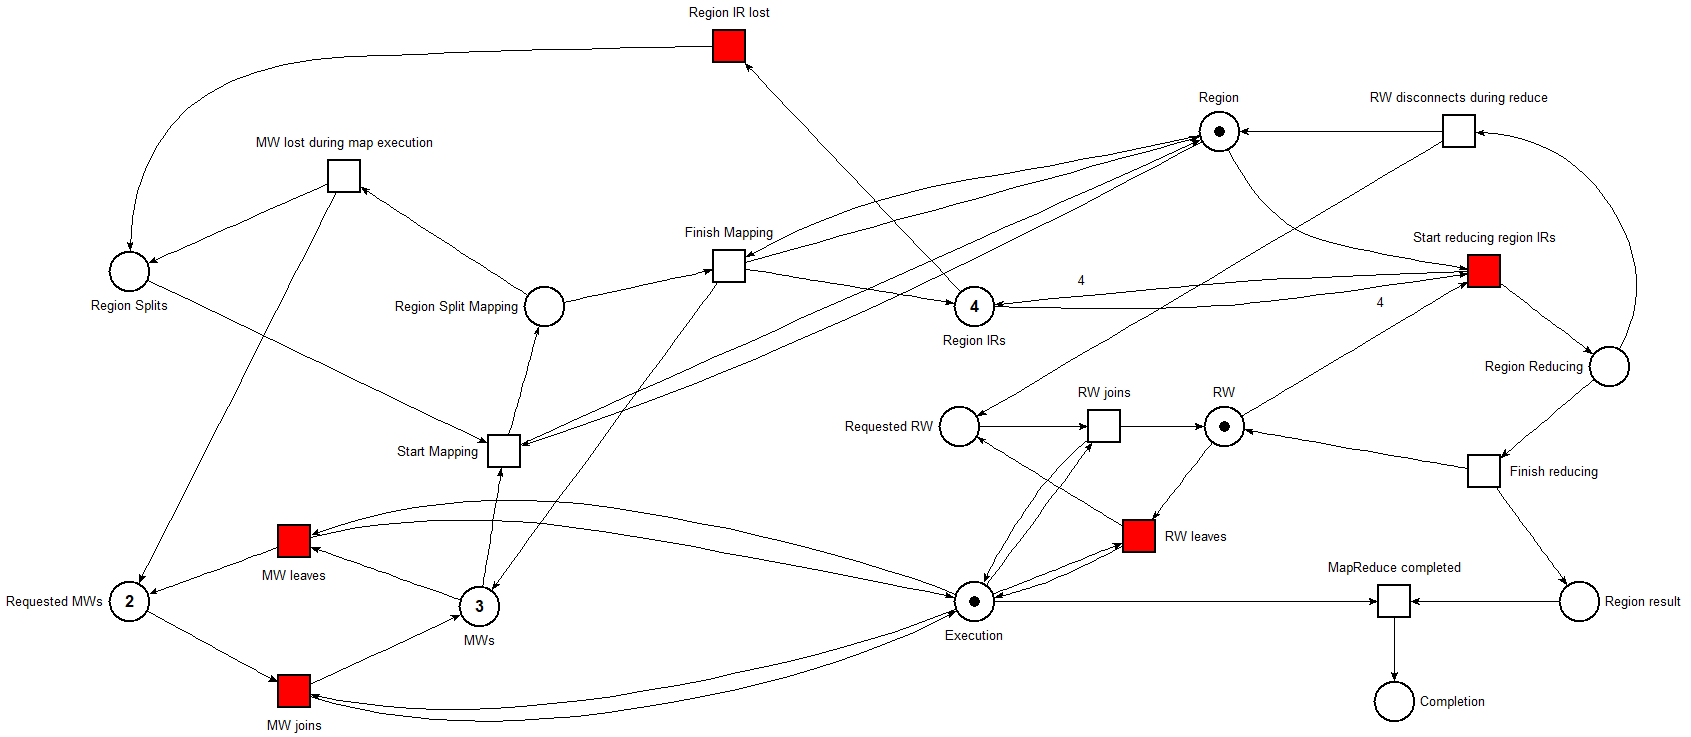
\includegraphics[width=\linewidth]{document/chapters/chapter_5/images/master_petri_net_3.png}
    \caption{MapReduce Master - Region Mapping completed}
    \label{fig:master_petri_net_3}
\end{figure}

While the reduce function is being applied, the region token is removed due to the fact that no more splits for this region need to be mapped (\textit{figure \ref{fig:master_petri_net_4}}). \textbf{A failure can also happen here, since the Reduce Worker can disconnect during the reduce function execution; in this case, the region token is restored and a new Reduce Worker is required}.

\vspace{5mm}

\begin{figure}[!ht]
    \centering
    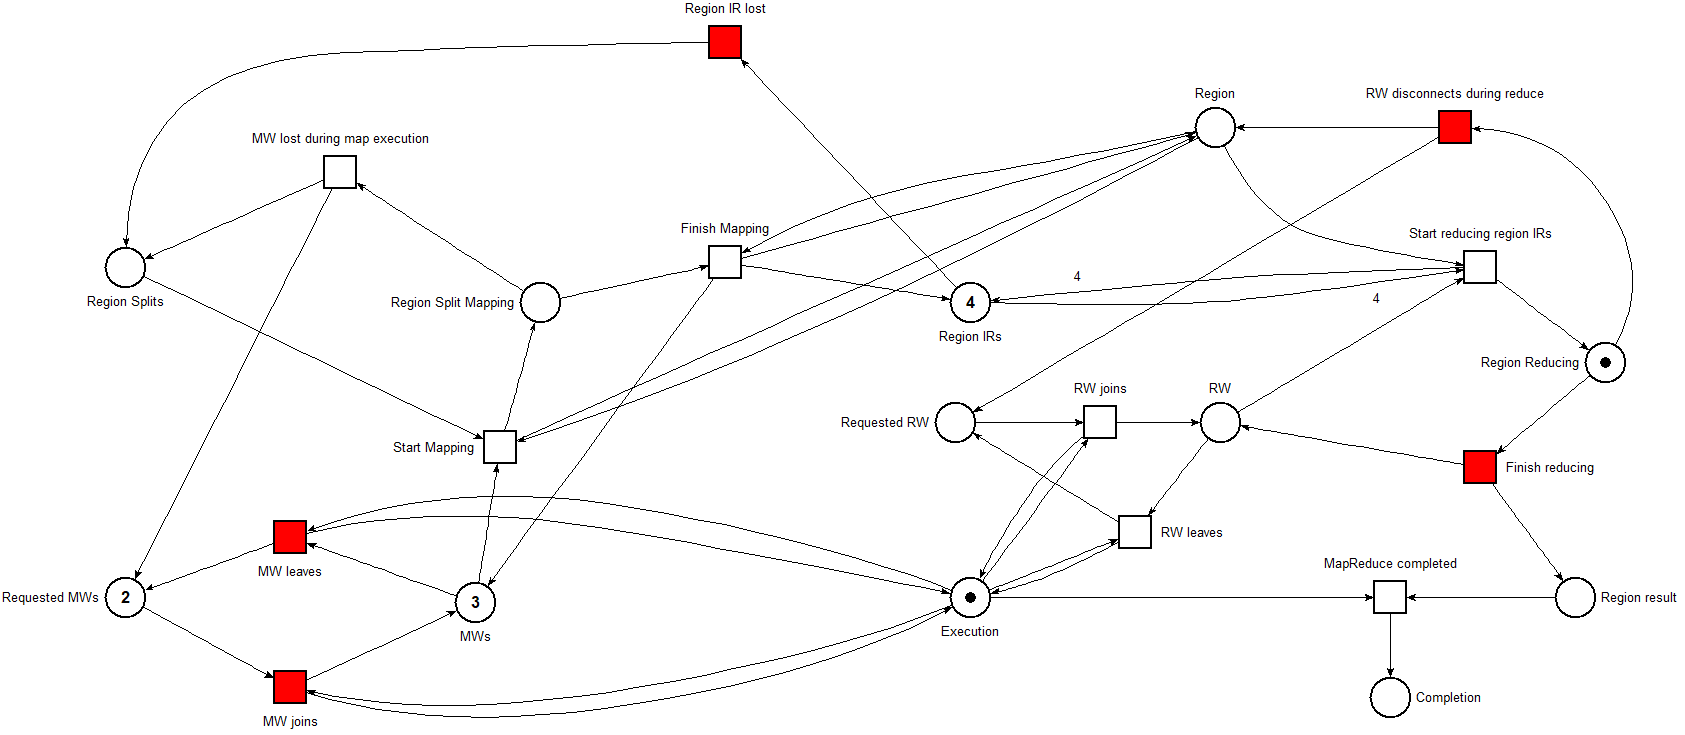
\includegraphics[width=\linewidth]{document/chapters/chapter_5/images/master_petri_net_4.png}
    \caption{MapReduce Master - Reducing process}
    \label{fig:master_petri_net_4}
\end{figure}

\textbf{If the reduce function is completed successfully} (as shown in \textit{figure \ref{fig:master_petri_net_5}}), \textbf{the region's result is obtained}. As stated before, the overall MapReduce execution will end once every region is computed, providing to the Customer all the regional results. 

\begin{figure}[!ht]
    \centering
    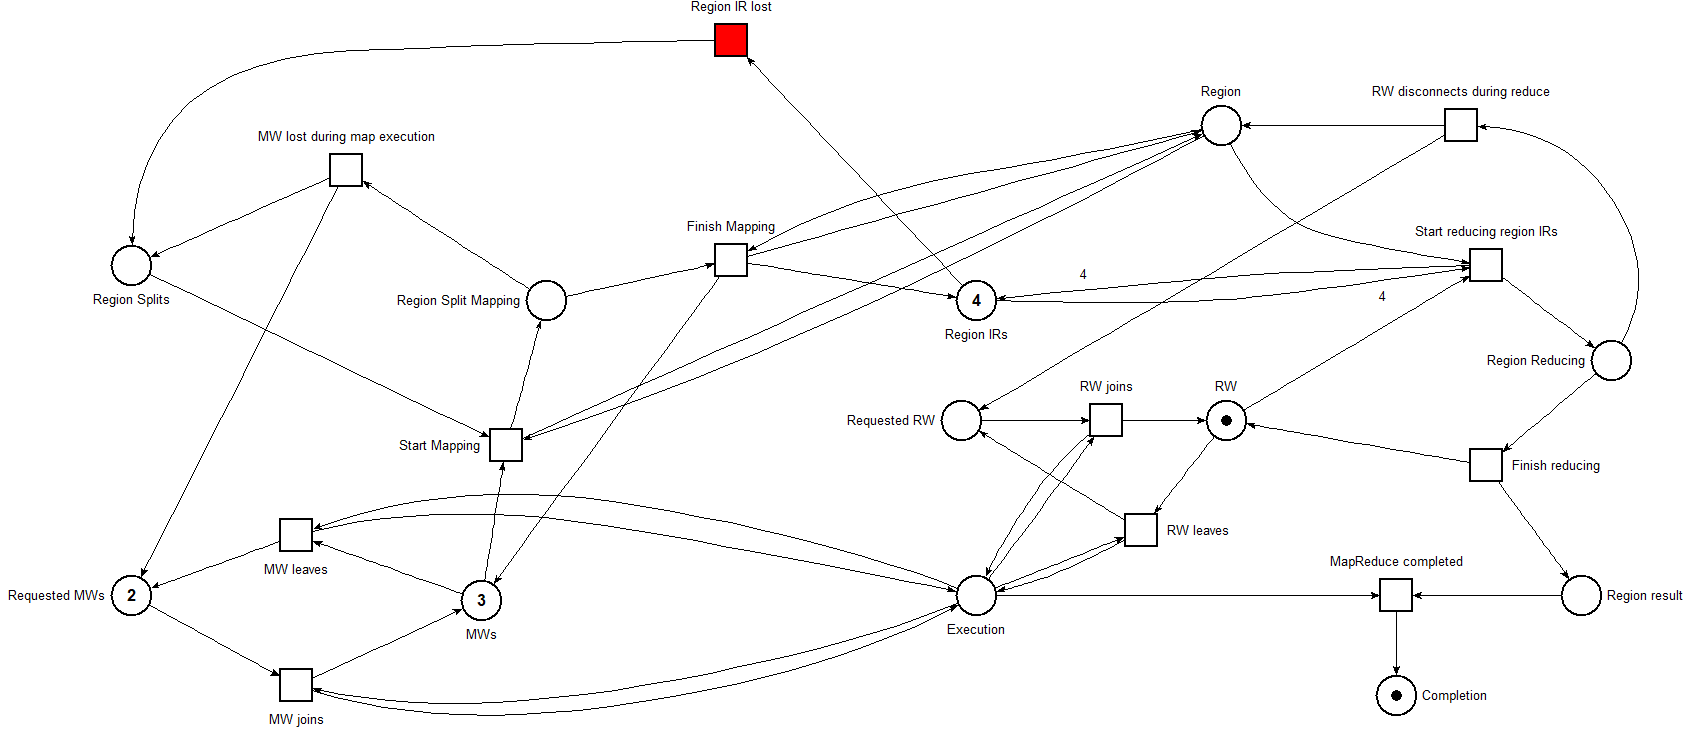
\includegraphics[width=\linewidth]{document/chapters/chapter_5/images/master_petri_net_5.png}
    \caption{MapReduce Master - Region completed}
    \label{fig:master_petri_net_5}
\end{figure}